\documentclass [10pt, fancyhdr, twoside] {article}
\usepackage{float, graphicx, caption, amssymb, natbib}
\usepackage[utf8]{vietnam}
\usepackage[usenames,dvipsnames]{color}
\usepackage{tabulary}
\usepackage [left=2.5cm, top=2.5cm, bottom=2.5cm, right=3cm] {geometry}  %% see geometry.pdf on how to lay out the page. There's lots.
\geometry{a4paper} %% or letter or a5paper or ... etc
\usepackage{fancyhdr}
\usepackage{xcolor}
\usepackage[scaled]{helvet}
\renewcommand*\familydefault{\sfdefault} %% Only if the base font of the document is to be sans serif

\usepackage[left]{lineno}


\pagestyle{fancy}

\fancyhead{}
\fancyfoot{}

\fancyhead[RO,LE]{Cắt và canh chỉnh ảnh căn cước công dân bằng YOLOv5}
\fancyfoot[RO,LE]{Page-\thepage}

\usepackage{blindtext}

\newcounter {note}
\stepcounter{note}

\renewcommand{\abstractname}{Abstract}


\begin{document}

\title{Cắt và canh chỉnh ảnh căn cước công dân bằng YOLOv5}
\author {Phan Đình Minh Hiếu - MSHV\: 220101024 (MSHV cũ\: 220104003)}
\date{{Ngày 10 tháng 3 năm 2023}}
\maketitle

\begin{abstract}
    Báo cáo này trình bày một phương pháp cắt và căn chỉnh ảnh bằng cách sử dụng mô hình YOLOv5 để phân vùng tượng trên ảnh kết hợp với hàm WrapPerspective để căn chỉnh căn cước công dân vào khung hình chuẩn, đồng thời cắt và xử lý ảnh để tạo ra những bức ảnh có kích thước nhỏ và ngay thẳng. Kết quả thực nghiệm cho thấy phương pháp này có thể giúp cải thiện đáng kể chất lượng và giảm được kích thước lưu trữ.
\end{abstract}

\section{Giới thiệu đề tài}
\subsection{EKYC}
eKYC là viết tắt của "Electronic Know Your Customer" là một quy trình xác thực khách hàng trực tuyến bằng các công nghệ điện tử và kỹ thuật số. Thông thường, các công ty tài chính, ngân hàng, các tổ chức tài chính khác sử dụng eKYC để đối chiếu thông tin của khách hàng mới đăng ký với các cơ sở dữ liệu tài chính có sẵn, giúp tiết kiệm thời gian và chi phí so với các phương thức truyền thống.

\begin{figure}[h]
    \caption{Electronic Know Your Customer}
    \centering
    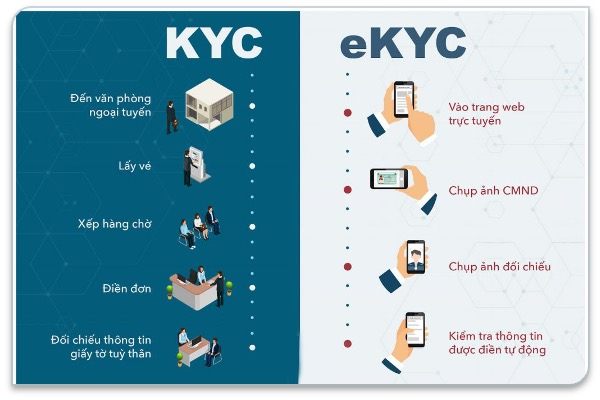
\includegraphics[width=15cm]{Picture1.jpg}
\end{figure}
\subsection{OCR}
Trong quy trình EKYC, OCR (Optical Character Recognition) là một công nghệ quan trọng được sử dụng để chuyển đổi các hình ảnh chứa các ký tự chữ và số sang các văn bản có thể xử lý được bằng máy tính. Các loại tài liệu mà OCR có thể xử lý bao gồm chứng minh thư, hộ chiếu, giấy phép lái xe, hóa đơn, giấy tờ tài chính và các tài liệu khác.

Trong quy trình EKYC, OCR được sử dụng để trích xuất thông tin từ các chứng minh thư, hộ chiếu và các tài liệu khác của khách hàng. Các thông tin này bao gồm họ tên, ngày sinh, số chứng minh thư, hộ chiếu và các thông tin khác cần thiết để xác thực danh tính của khách hàng. OCR giúp giảm thiểu thời gian và chi phí của quy trình xác thực, đồng thời giảm thiểu các sai sót do việc nhập liệu thủ công.

\begin{figure}[h]
    \caption{Optical Character Recognition}
    \centering
    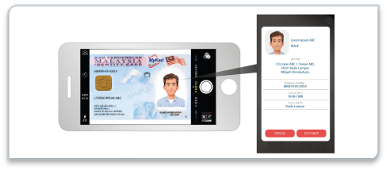
\includegraphics[width=10cm]{Picture2.png}
\end{figure}

\subsection{Giới thiệu đề tài}
Chức năng của đề tài "Cắt và Canh chỉnh thẻ căn cước cá nhân đối với EKYC và OCR" là tối ưu hóa quy trình xác thực danh tính trong quy trình EKYC bằng cách tự động cắt và canh chỉnh hình ảnh chứa các thẻ căn cước cá nhân trước khi áp dụng OCR. Điều này giúp đảm bảo độ chính xác và hiệu quả của quy trình trích xuất thông tin từ hình ảnh đồng thời giảm kích thước lưu trữ dữ liệu.

\section{Phương pháp}
\subsection{Sử dụng YOLOv5 để phân vùng ảnh}
Yolov5 (You Only Look Once version 5) là một mô hình nhận diện vật thể dựa trên Deep Learning, được phát triển bởi đội ngũ của Ultralytics. Yolov5 là phiên bản nâng cấp của Yolov4, được giới thiệu vào năm 2020.
Mô hình Yolov5 có thể dùng cho bài toán phân vùng ảnh với nhiều vật thể khác nhau.\\
\begin{figure}[h]
    \caption{YOLOv5 được dùng để phân vùng ảnh}
    \centering
    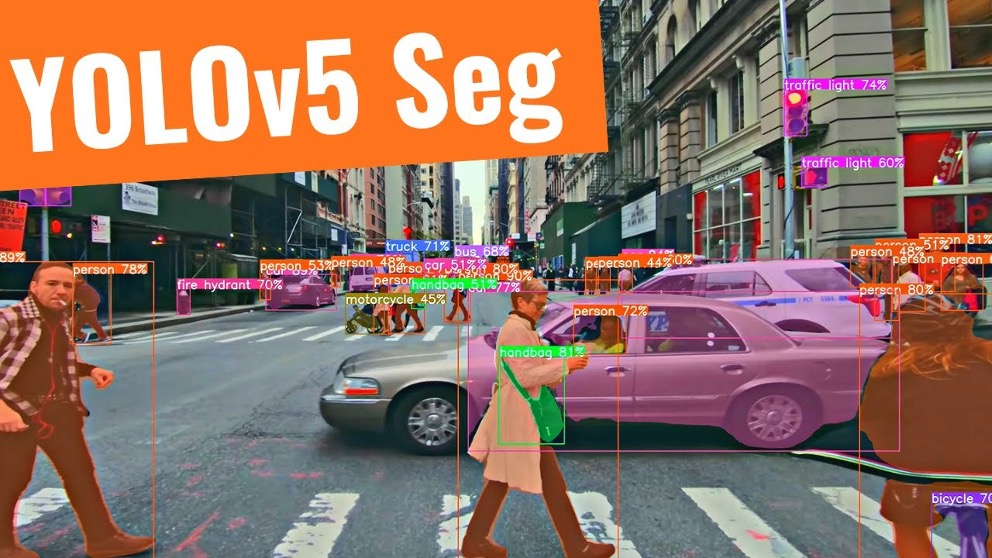
\includegraphics[width=10cm]{Picture3.jpg}
\end{figure}

\pagebreak
Báo cáo này sử dụng tham số pretrain YOLOv5n nhằm mục đích tạo ra một model gọn nhẹ để có thể chạy được trên các thiết bị di động từ đó tăng tính áp dụng vào thực tế
\begin{figure}[h]
    \caption{Các mô hình pretrain của YOLOv5}
    \centering
    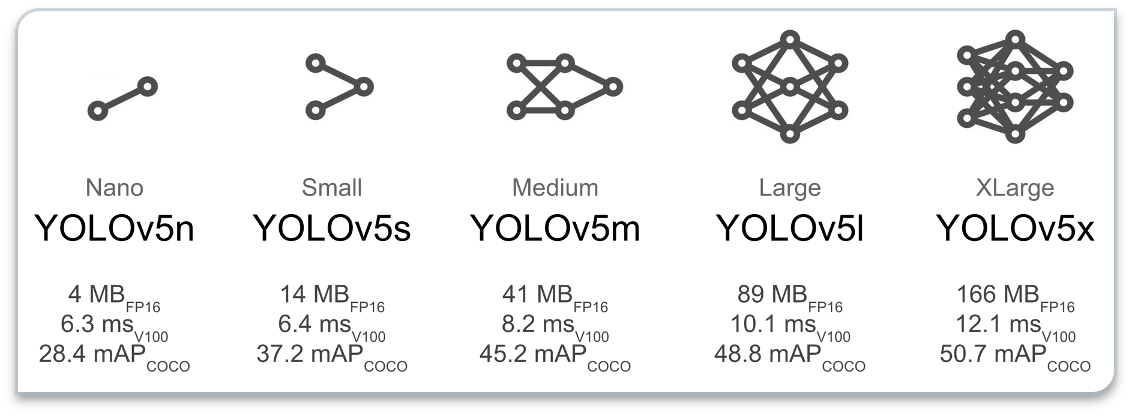
\includegraphics[width=10cm]{Picture4.png}
\end{figure}


Sau khi sử dụng yolo để phân đoạn hình ảnh, chúng ta sẽ có được mask của hình căn cước công dân. Từ mask này chúng ta đến với bước tiếp theo để hoàn thành việc cắt và căn chỉnh ảnh căn cước công dân.
\subsection{Xoay hình với hàm WrapPerspective}
 Hàm WrapPerspective là một trong những hàm quan trọng trong thư viện xử lý ảnh OpenCV. Hàm này được sử dụng để áp dụng phép biến đổi affine hoặc phép biến đổi hình học phức tạp trên một ảnh hoặc một tập hợp các điểm trong không gian 2D.
\\
 Phép biến đổi affine là một phép biến đổi toán học dùng để di chuyển, xoay, co giãn hay góc phóng hình ảnh. Nó được định nghĩa bởi một ma trận 3x3 và có thể được sử dụng để biến đổi tất cả các điểm trong ảnh hoặc tập hợp các điểm trên mặt phẳng 2D.
\\
 Hàm WrapPerspective sử dụng phép biến đổi affine để thực hiện việc căn chỉnh và xoay các đối tượng trong ảnh, đồng thời cắt ảnh theo kích thước và vị trí mong muốn. Hàm này có đầu vào là ảnh cần được xử lý, ma trận 3x3 mô tả phép biến đổi affine và kích thước của ảnh kết quả.
\\
Khi được áp dụng cho các ảnh chứa đối tượng cần phát hiện, hàm WrapPerspective có thể giúp căn chỉnh đối tượng vào khung hình chuẩn và giảm thiểu các sai lệch và nhiễu trong ảnh. Điều này giúp tăng độ chính xác của việc phát hiện đối tượng và cải thiện chất lượng của ảnh.
\begin{figure}[h]
    \caption{Mô tả hàm WrapPerspective}
    \centering
    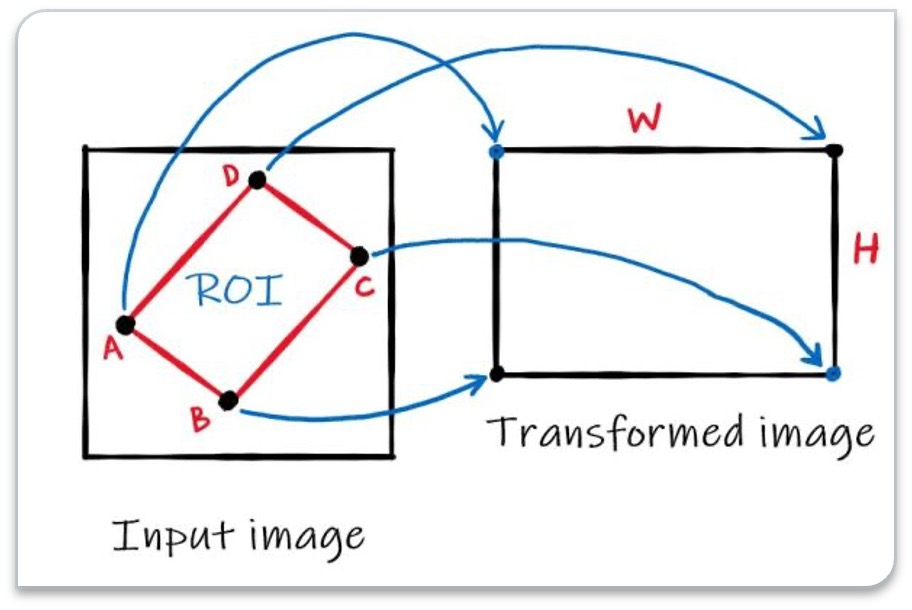
\includegraphics[width=10cm]{Picture5.jpg}
\end{figure}


Sau khi đã cắt và xoay ảnh xong, sẽ có trường hợp ảnh bị ngược 180 độ, khi đó ta sẽ tiến hành phát hiện thêm đối tượng là hình chụp chân dung. Nếu hình chụp chân dung nằm bên phải thì ta sẽ tiến hành xoay hình 180 độ để có được hình đúng. 
\section{Kết quả}
\subsection{Môi trường thực nghiệm}
Hệ điều hành: macOS 13.2.1 \\
Mô hình: YOLOv5 v7.0-120-g3e55763 \\ 
Phiên bản Python: Python-3.9.6 \\
Phiên bản pyTorch: torch-2.1.0.dev20230313 \\
Số vòng lăp: 50 epochs \\
Số mẫu dữ liệu: 257 hình (217 train, 55 validate)
\subsection{Độ đo}
\begin{tabular}{|p{1.25in}|p{1.25in}|p{1.25in}|} 
    \hline
    mAp & Accuracy & Recall\\
    \hline
    0.82 & 0.95 & 0.85
    \\ 
    \hline
\end{tabular}

\subsection{Chạy mẫu}
\begin{figure}[h]
   
    \centering
    
    
\end{figure}

\begin{figure}[!htb]
    \begin{minipage}{0.48\textwidth}
      \caption{Hình gốc}
      \centering
      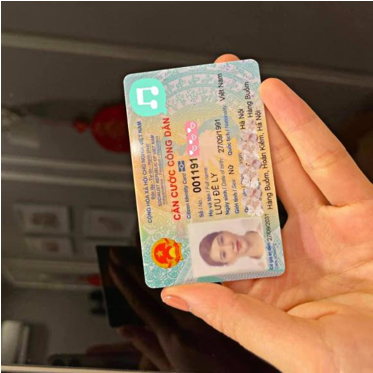
\includegraphics[width=7cm]{Picture6.png}
    \end{minipage}\hfill
    \begin{minipage}{0.48\textwidth}
      \centering
      \caption{Kết quả sau khi chạy}
      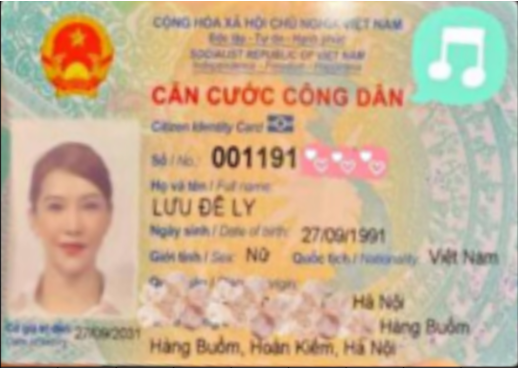
\includegraphics[width=7cm]{Picture7.png}
    \end{minipage}
 \end{figure}

\section{Kết luận}
Tổng kết lại, bài báo cáo này đã trình bày một phương pháp cắt và căn chỉnh ảnh bằng cách sử dụng phân đoạn ảnh với mô hình YOLOv5 kết hợp với hàm WrapPerspective để thực hiện phép biến đổi affine trên ảnh và cắt ảnh theo kích thước, vị trí mong muốn.

Kết quả thực nghiệm cho thấy phương pháp này có thể cải thiện đáng kể chất lượng ảnh và độ chính xác của việc phát hiện đối tượng trên ảnh. Phương pháp này đã giúp giảm thiểu các sai lệch và nhiễu trong ảnh, tạo ra những bức ảnh có chất lượng cao trước khi bắt đầu quá trình OCR cũng như giảm thiểu dung lượng lưu trữ ảnh.

Phương pháp này có thể được áp dụng rộng rãi trong nhiều lĩnh vực khác nhau, bao gồm nhận diện giấy tờ, phân tích ảnh y khoa, giám sát an ninh, v.v. Tuy nhiên, việc áp dụng phương pháp này cần phải cân nhắc kỹ lưỡng đến các yếu tố về các đặc trưng cần thiết để có thể xoay ảnh được đúng như ý muốn.


\end{document}